% ****** Start of file apssamp.tex ******
%
%   This file is part of the APS files in the REVTeX 4.1 distribution.
%   Version 4.1r of REVTeX, August 2010
%
%   Copyright (c) 2009, 2010 The American Physical Society.
%
%   See the REVTeX 4 README file for restrictions and more information.
%
% TeX'ing this file requires that you have AMS-LaTeX 2.0 installed
% as well as the rest of the prerequisites for REVTeX 4.1
%
% See the REVTeX 4 README file
% It also requires running BibTeX. The commands are as follows:
%
%  1)  latex apssamp.tex
%  2)  bibtex apssamp
%  3)  latex apssamp.tex
%  4)  latex apssamp.tex
%
\documentclass[%
 reprint,	
%superscriptaddress,
%groupedaddress,
%unsortedaddress,
%runinaddress,
%frontmatterverbose, 
%preprint,
showpacs,
% preprintnumbers,
%nofootinbib,
%nobibnotes,
%bibnotes,
 amsmath,amssymb,
 aps,
 prc,
%prb,
%rmp,
%prstab,
%prstper,
%floatfix,
]{revtex4-1}

\usepackage{graphicx}% Include figure files
\usepackage{dcolumn}% Align table columns on decimal point
\usepackage{bm}% bold math
\usepackage{url}
\usepackage{lipsum}
\usepackage{color}
\usepackage{hyperref}% add hypertext capabilities
\usepackage[mathlines]{lineno}% Enable numbering of text and display math
\usepackage{upgreek}
\usepackage{biolinum}
% \linenumbers\relax % Commence numbering lines

%\usepackage[showframe,%Uncomment any one of the following lines to test 
%%scale=0.7, marginratio={1:1, 2:3}, ignoreall,% default settings
%%text={7in,10in},centering,
%%margin=1.5in,
%%total={6.5in,8.75in}, top=1.2in, left=0.9in, includefoot,
%%height=10in,a5paper,hmargin={3cm,0.8in},
%]{geometry}

% \setcounter{secnumdepth}{5}
\begin{document}

\preprint{APS/123-QED}

\title{Measurement of $\phi$-meson Production in Au+Au Collisions at ${\sqrt{s_{\rm NN}} = \rm{3\,GeV}}$}% Force line breaks with \\
%\thanks{A footnote to the article title}%

% \author{Ann Author}
% \altaffiliation[Also at ]{Physics Department, XYZ University.}%Lines break automatically or can be forced with \\
% \author{Second Author}%
% \email{Second.Author@institution.edu}
% \affiliation{% Authors' institution and/or address\\ This line break forced with \textbackslash\textbackslash
% }%

\collaboration{STAR Collaboration}
\noaffiliation

\date{\today}% It is always \today, today,
             %  but any date may be explicitly specified

\begin{abstract}


We report on the first measurement of $\phi$-meson production and $\phi/K^-$ ratio in Au+Au collisions at ${\sqrt{s_{\rm NN}} = \rm{3\,GeV}}$ with RHIC/STAR experiment under fixed target configuration. $\phi$-mesons are measured through their hadronic decay channel, $\phi\rightarrow K^+K^-$. The transverse momentum ($p_T$) spectra of $\phi$-mesons and $K^-$ are presented in different centrality and rapidity intervals. The total production yields and $\phi/K^-$ ratio in $4\pi$ acceptance are calculated and compared to thermal model predictions. The grand canonical ensemble (GCE) calculation shows a clear discrepancy from our measurement. Our data favors the canonical ensemble (CE) model with a strangeness correlation length $(r_c   \sim 3.2_{-0.1}^{+0.4} \rm{fm})$ in 0-10\% central Au+Au collisions at ${\sqrt{s_{\rm NN}} = \rm{3\,GeV}}$.


%\begin{description}
%\item[Usage]
%Secondary publications and information retrieval purposes.
%\item[PACS numbers]
%May be entered using the \verb+\pacs{#1}+ command.
%\item[Structure]
%You may use the \texttt{description} environment to structure your abstract; use the optional argument of the \verb+\item+ command to give the category of each item. 
%\end{description}
\end{abstract}

\pacs{25.75.-q, 25.75.Cj}% PACS, the Physics and Astronomy
                             % Classification Scheme.
%\keywords{Suggested keywords}%Use showkeys class option if keyword
                              %display desired
\maketitle

% Chapter one
% \section{Introduction}
% \label{introduction}

Relativistic heavy ion physics is aimed for detail investigation of phase structures of strongly interacting matter, governed by Quantum Chromodynamics (QCD), under extreme high temperature and density conditions. 


Recently measurements of $\phi$-meson over $K^-$ ratio in heavy-ion collisions show a relative enhancement in the low energies below the NN threshold compare to the high energies at RHIC and LHC. These enhancement were observed both in Au+Au collisions and also in the lighter system such as Ni+Ni, Ar+KCl and Al+Al at low energies. The grand canonical ensemble (GCE) statistical model shows a discrepancy with the measured data while the calculations from canonical ensemble (CE) with different strangeness correlation length ($r_c$) can reasonable reproduce this feature. In the GCE, the strangeness was conserved in average for the collision system, while the $r_c$ parameter in CE model corresponding to the strangeness local conserved volume size. Due to the uncertainties in the current measurements, a solid determination on the $r_c$ and distinguish those different models are still missing. The Fixed-Target program at STAR covers the center-of-mass energy (cms) from 3.0 GeV to 7.7 GeV which can map the unmeasured cms range to have a better constrain on the model calculations~\cite{}.


% The dataset used in this analysis consists of Au+Au collision events at ${\sqrt{s_{\rm NN}} = \rm{3\,GeV}}$ collected in the 2018 RHIC run. The main detectors used are the Time Projection Chamber (TPC), the HFT, the Time of Flight (TOF) detector, and the Vertex Position Detector (VPD). 


% Particle tracking for this analysis is achieved with the TPC and HFT detectors. The HFT detector provides measured space points with high precision that are used to extend track trajectories from the TPC and offer high-pointing resolution to the vicinity of the event vertex. Particle identification is achieved with a combination of the ionization energy loss ($dE/dx$) measurement with the TPC and the time-of-flight ($tof$) measurement with the TOF detector. The event start time is provided by the VPD. Both the TPC and TOF detectors have full azimuthal coverage with a pseudo-rapidity range of $|\eta|$\,$<$\,1~\cite{TPC,TOF}. The TPC and TOF subsystems have been extensively used in many prior STAR analyses, including $D$-meson measurements ~\cite{Star_D_pp,Star_D_RAA,Adamczyk:2015ukd}.


% The minimum bias trigger is defined as a coincidence between the east and west VPD detectors located at 4.4\,$<$\,$|\eta|$\,$<$\,4.9~\cite{VPD}. Each VPD detector is an assembly of nineteen small detectors, each consisting of a Pb converter followed by a fast plastic scintillator read out by a photomultiplier tube. To efficiently sample the collision events in the center of the HFT acceptance, an online cut on the collision vertex position along the beam line (calculated via the time difference between the east and west VPD detectors) $|V_z^{\rm VPD}|$\,$<$\,6\,cm is applied. 

% Events are selected with the offline reconstructed collision vertex ~\cite{Smirnov_2017} within 6 cm of the TPC and HFT centers along the beam direction to ensure uniform and large acceptance. Event pileup due to the long TPC readout time ($\approx$\,40\,$\upmu$s) with respect to the Au-Au collision rate (40 KHz) is rejected by removing events that have an online and offline vertex position difference along the z-axis ($|V_z^{\rm VPD}-V_z^{\rm TPC}|$) greater than 3 cm. Approximately 9$\times 10^{8}$ minimum bias triggered events with 0--80\% centrality pass the selection criteria and are used in this analysis.


% $D^0$ and $\overline{D}^{0}$ mesons are reconstructed via the hadronic decay channel $D^0\rightarrow K^-\pi^+$ and its charge conjugate channel with a branching ratio ($B.R.$) of 3.89\%~\cite{pdg}. In what follows, we imply $(D^0 +\overline{D}^{0})/2$ when using the term $D^0$ unless otherwise specified. $D^0$ mesons decay with a proper decay length of $c\tau$ $\approx$\,123\ $\upmu$m after they are produced in Au+Au collisions. We utilize the high-pointing resolution capability enabled by the HFT detector to topologically reconstruct the $D^0$ decay vertices that are separated from the collision vertices, which drastically reduces the combinatorial background (around five orders of magnitude) and improves the measurement precision.

% Charged pion and kaon tracks are reconstructed with the TPC and HFT. Tracks are required to have at least 20 measured TPC points out of maximum 45 to ensure a good momentum resolution. To enable high pointing precision, both daughter tracks are required to have at least one measured hit in each layer of the PXL and IST as described above. Particle identification is achieved via a combination of the ionization energy loss measurement in the TPC and the time-of-flight measurement in the TOF. The resolution-normalized $dE/dx$ deviation from the expected values is defined as:
% \begin{equation}
%   n\sigma_X = \frac{1}{R}\ln\frac{\langle{dE/dx}\rangle_{\rm {mea.}}}{\langle{dE/dx}\rangle_{X}},
% \label{equ:equation1}
% \end{equation}
% where $\langle{dE/dx}\rangle_{\rm {mea.}}$ and $\langle{dE/dx}\rangle_{X}$ represent measured and expected values with a hypothesis of particle $X$, and $R$ is the $dE/dx$ resolution (typically $\approx$\,8\%~\cite{TPC}). The $n\sigma_X$ distribution should be close to a standard Gaussian for each corresponding particle species (mean $=$ 0, $\sigma = $ 1) with good $dE/dx$ calibration.
% Pion (kaon) candidates are selected by a requirement of the measured $dE/dx$ to be within three (two) standard deviations ($|n\sigma_{X}|$) from the expected value. When tracks have matched hits in the TOF detector, an additional requirement on the measured inverse particle velocity ($1/\beta$) to be within three standard deviations from the expected value ($|\Delta 1/\beta|$) is applied for either daughter track. Figures~\ref{fig:PID_dEdx} and ~\ref{fig:PID_beta} show examples of the particle identification capability from the TPC and TOF. Tracks within the kinematic acceptance $p_{T}$\,$>$\,0.6\,GeV/$c$ and $|\eta|$\,$<$\,1 are used to combine and make pairs. The choice of the $p_T$\,$>$\,0.6\,GeV/$c$ cut is an optimized consideration to balance the loss of signal acceptance when tightening the cut, and the increase in background due to the HFT fake matches when loosening this cut (see Sec.~\ref{correction:hft}). The threshold has been varied for systematic uncertainty evaluation. See Sec.~\ref{systematic} for details. Table~\ref{table:singlecut} lists the TPC and TOF selection cuts for daughter kaon and pion tracks used for $D^0$ reconstruction.


% \begin{figure*}
% \centering
% \includegraphics[width=1.0\textwidth]{fig/signal_0_8_10GeV.pdf}
% \caption{Invariant mass $M_{K\pi}$ distributions in 0\,$<$\,$p_{T}$\,$<$\,10\,GeV/$c$ from centrality bins 0--80\% (a), 0--10\% (b), and in 0\,$<$\,$p_{T}$\,$<$\,8\,GeV/$c$ for 60--80\% (c), respectively. Black open circles represent the same-event (SE) unlike-sign (US) distributions. Blue and grey shaded histograms represent the SE like-sign (LS) and mixed-event (ME) US distributions that are used to estimate the combinatorial background. The red solid circles depict the US (SE) distributions with the combinatorial background subtracted using the US (ME) distributions.
% }
% \label{fig:signal_0} 
% \end{figure*}
%
% Figure~\ref{fig:signal_0} shows the invariant mass distributions of $K\pi$ pairs in the $p_{T}$ region of 0--10 GeV/$c$ for 0--80\% minimum bias and the 0--10\% most central collisions, and 0--8 GeV/$c$ for 60--80\% peripheral collisions, respectively. The reason of choosing a different $p_T$ range for the 60--80\% centrality bin is because no signal is observed beyond the current statistics. The combinatorial background is estimated with the same-event (SE) like-sign (LS) pairs (blue histograms) and the mixed-event (ME) unlike-sign (US) (grey histograms) technique in which $K$ and $\pi$ from different events of similar characteristics ($V_{Z}$, centrality, event plane angle) are paired. The mixed-event spectra are normalized to the like-sign distributions in the mass range of 1.7--2.1\,GeV/$c^2$. After the subtraction of the mixed-event unlike-sign combinatorial background from the same-event unlike-sign pairs (black open circles), the remainder distributions are shown as red solid circles in each panel. Compared to the previous $D^0$ measurement~\cite{Star_D_RAA}, the $D^0$ signal significance is largely improved by a factor of $\approx$\,15 using the same amount of event statistics. 
%
%
% After the combinatorial background is subtracted, the residual $K\pi$ invariant mass distributions are fit to a Gaussian plus linear function. The linear function is used to represent remaining correlated background from either partial reconstruction of charm mesons or jet fragments.
% The $D^0$ raw yields are extracted from the Gaussian function fit results and the systematic uncertainty on the extracted raw yield is evaluated using several methods described in Sec.~\ref{systematic}.
%
%
% The reconstructed $D^0$ raw yields are calculated in each centrality and $p_{T}$ bin within the rapidity window $|y|$\,$<$\,1. The fully corrected $D^0$ production invariant yields are calculated using the following formula:
% \begin{equation}
%   \begin{aligned}
% & \frac{d^2N}{2\pi p_{T}dp_{T}dy} = \frac{1}{\rm B.R.} \times \frac{N^{\rm raw}}{N_{\rm evt} 2\pi p_{T}\Delta p_{T}\Delta y} \\
% & \times \frac{1}{\varepsilon_{\rm trg}\times\varepsilon_{\rm TPC}\times\varepsilon_{\rm HFT}\times\varepsilon_{\rm PID}\times\varepsilon_{\rm vtx}},
%   \end{aligned}
% \label{equ:invariantyield}
% \end{equation}
% where B.R. is the $D^0\rightarrow K^-\pi^+$ decay branching ratio, (3.89$\pm$0.04)\%~\cite{pdg}, $N^{\rm raw}$ is the reconstructed $D^0$ raw counts, $N_{\rm evt}$ is the total numbers of events used in this analysis, and $\varepsilon_{\rm trg}$ is the centrality bias correction factor described in Sec.~\ref{dataset:trigger}. The raw yields are corrected for the TPC acceptance and tracking efficiency - $\varepsilon_{\rm TPC}$, the HFT acceptance and tracking plus topological cut efficiency - $\varepsilon_{\rm HFT}$, the particle identification efficiency - $\varepsilon_{\rm PID}$, and the finite vertex resolution correction - $\varepsilon_{\rm vtx}$.


% The systematic uncertainty on the final measured $D^0$ $p_{T}$ spectra can be categorized as the uncertainty of the raw $D^0$ yield extraction, the BR uncertainty, and the uncertainty of efficiencies and corrections.

% The uncertainty of the raw yield extraction is estimated by a) changing the $D^0$ raw yield counting method from the Gaussian fit to histogram bin counting. b) varying invariant mass ranges for fit and for side bands and c) varying background estimation between the mixed-event and like-sign methods. For the side band method, the $D^0$ raw yield is obtained by subtracting the average counts in two invariant mass ranges around the signal (1.71--1.80 and 1.93--2.02 GeV/$c^2$) from the counts in the signal region (1.82--1.91 GeV/$c^2$)~\cite{Star_D_v2,Star_D_pp}. The maximum difference between these scenarios is then converted to the standard deviation and added to the systematic uncertainties. It is the smallest in the mid-$p_{T}$ bins due to the best signal significance and grows at both low and high $p_{T}$. The double counting contribution in the $D^0$ raw yield  due to mis-PID is included as another contribution to the systematic uncertainty for the $D^0$ raw yield extraction as described in Sec.~\ref{correction:PID}.

% The uncertainty of the TPC acceptance and efficiency correction $\varepsilon_{\rm TPC}$ is estimated via the standard procedure in STAR by comparing the TPC track distributions between real data and the embedding data. It is estimated to be $\approx$\,5--7\% for 0--10\% collisions and $\approx$\,5--8\% for 60--80\% collisions, and is correlated for different centralities and $p_{T}$ regions. 

% The uncertainty of the PID efficiency correction is estimated by varying the PID selection cuts and then convoluting to the final corrected $D^0$ yield. 


% To estimate the uncertainty of the HFT tracking and topological cut efficiency correction $\varepsilon_{\rm HFT}$, we employ the following procedures: a) We vary the topological variable cuts such that the $D^0$ $\varepsilon_{\rm HFT}$ is changed to 50\% and 150\% from the nominal (default) efficiency and compare the efficiency--corrected final $D^0$ yields. The maximum difference between the two scenarios is then added to the systematic uncertainties. b) We also vary the lower threshold cut on the daughter $p_{T}$ between 0.3 to 0.6 GeV/$c$ and the maximum difference in the final corrected $D^0$ yield is also included in the systematic uncertainties. c) We add the systematic uncertainty due to limitation of the data-driven simulation approach, $\approx$\,5\%, and the impact of the secondary particles, $\approx$\,2\%, to the total $\varepsilon_{\rm HFT}$ systematic uncertainty.
%
% With the corrected $D^0$ transverse momentum spectra, the nuclear modification factor $R_{\rm CP}$ is calculated as the ratio of $N_{\rm bin}$--normalized yields between central and peripheral collisions, as shown in the following formula:
% \begin{equation}
%   R_{\rm CP} = \frac{d^2N/dp_{T}dy}{N_{\rm bin}} |_{\rm cen\ } \times \frac{N_{\rm bin}} {d^2N/dp_{T}dy} |_{\rm peri }.
% \label{equ:equation3}
% \end{equation}
%
% The systematic uncertainties in the raw signal extraction in central and peripheral collisions are propagated as they are uncorrelated, while the systematic uncertainties from the other sources are correlated or partially correlated in contributing to the measured $D^0$ yields. To study these correlations, we vary selection cuts simultaneously in central and peripheral collisions, and the difference in the final extracted $R_{\rm CP}$ value is then directly counted as systematic uncertainties in the measured $R_{\rm CP}$.
%
% The nuclear modification factor $R_{\rm AA}$ is calculated as the ratio of $N_{\rm bin}$--normalized yields between Au+Au and $p$+$p$ collisions. The baseline for $p$+$p$ collisions is the same as in Ref.~\cite{Star_D_RAA}. The uncertainties from the $p$+$p$ reference dominates the systematic uncertainty for $R_{\rm AA}$. They include the 1$\sigma$ uncertainty from the Levy function fit to the measured spectrum and the difference between Levy and power-law function fits for extrapolation to low and high $p_T$, expressed as one standard deviation.
%
% With the corrected $D^0$ and $\overline{D}^{0}$ transverse momentum spectra, the $\overline{D}^{0}/D^0$ ratio is calculated as a function of the transverse momentum. The systematic uncertainties in the raw signal extraction for $\overline{D}^{0}$ and $D^0$ are propagated as they are uncorrelated, while the systematic uncertainties from the other sources are correlated or partially correlated in contributing to the measured $\overline{D}^{0}/D^0$ ratio. As in the $R_{\rm CP}$ systematic uncertainty estimation, we vary selection cuts simultaneously for $D^0$ and $\overline{D}^{0}$, and the difference in the final extracted $\overline{D}^{0}/D^0$ value is then directly counted as systematic uncertainties for the measured $\overline{D}^{0}/D^0$ ratio.


% \subsection{$p_{T}$ Spectra and Integrated Yields}
% \label{result:pt}

% Figure~\ref{fig:D0_spectra} shows the efficiency--corrected $D^0$ invariant yield at mid-rapidity ($|y|<1$) as a function of $p_{T}$ in 0--10\%, 10--20\%, 20--40\%, 40--60\% and 60--80\% Au+Au collisions. $D^0$ spectra in some centrality bins are scaled with arbitrary factors indicated on the figure for clarity. Dashed and solid lines depict fits to the spectra with the Levy function:
%
% where $m_0$ is the $D^0$ mass (1.864 GeV/$c^2$) and $dN/dy$, $T$ and $n$ are free parameters. The Levy function fit describes the $D^0$ spectra nicely in all centrality bins in our measured $p_T$ region.


% \begin{figure}
% \centering
% \includegraphics[width=0.43\textwidth]{fig/D0_spectra.eps}
% \caption{$D^{0}$ invariant yield at mid-rapidity ($|y|<1$) vs. transverse momentum for different centrality classes. Error bars (not visible for many data points) indicate statistical uncertainties and brackets depict systematic uncertainties. Global systematic uncertainties in $B.R.$ are not plotted. Solid and dashed lines depict Levy function fits.}
% \label{fig:D0_spectra} 
% \end{figure}




\begin{figure}
\centering
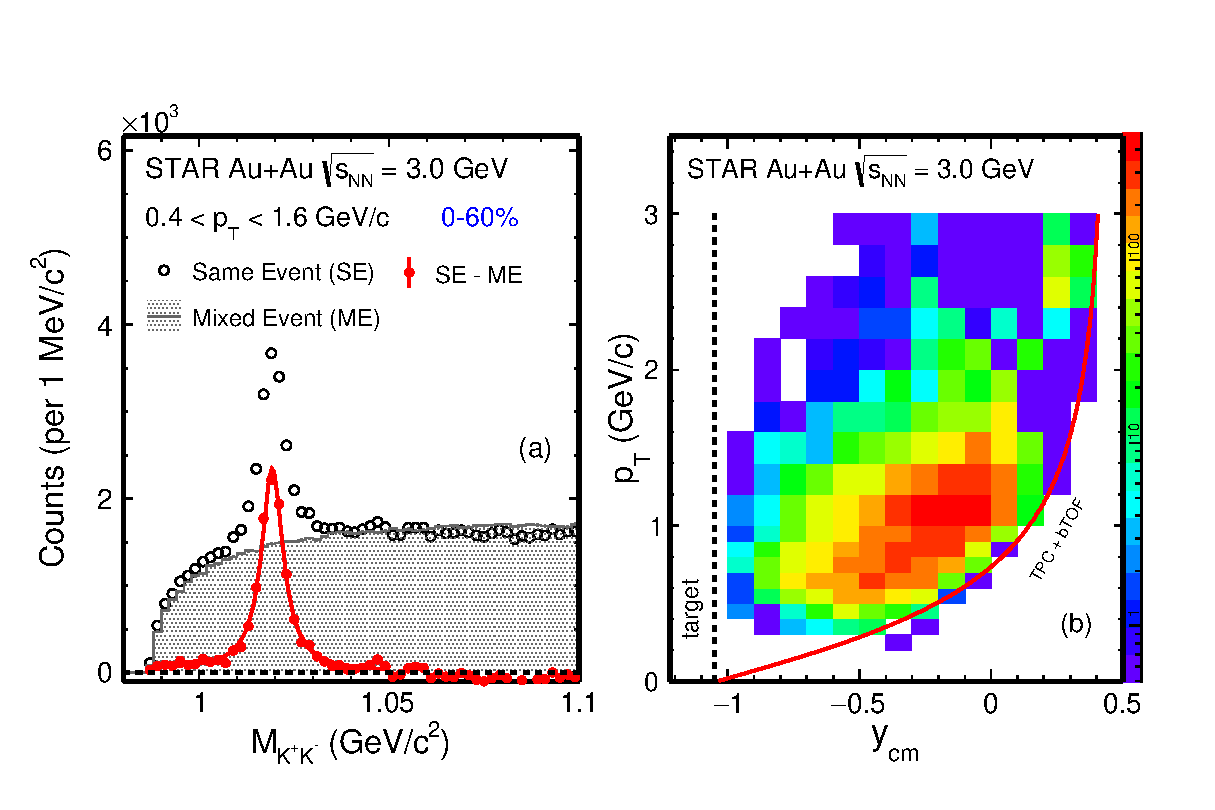
\includegraphics[width=0.50\textwidth]{fig/fig1_signal.eps}
  \caption{(a) Invariant mass of $K^+K^-$ pairs in 0-60\% centrality and 0.4--1.6\,GeV/$c$. Black open circles represent the same-event (SE) unlike-sign (US) distributions. Grey shaded histograms represent the mix-event (ME) US distributions that are used to estimate the combinatorial background. The red solid circles depict the $\phi$-meson signals obtained by subtracting the ME combinatorial background from the SE distributions. (b) The reconstructed $\phi$-meson acceptance $p_T$ vs. rapidity in the center-of-mass frame ($y_{\rm cm}$).}
\label{fig:phiSignal} 
\end{figure}

\begin{figure}
\centering
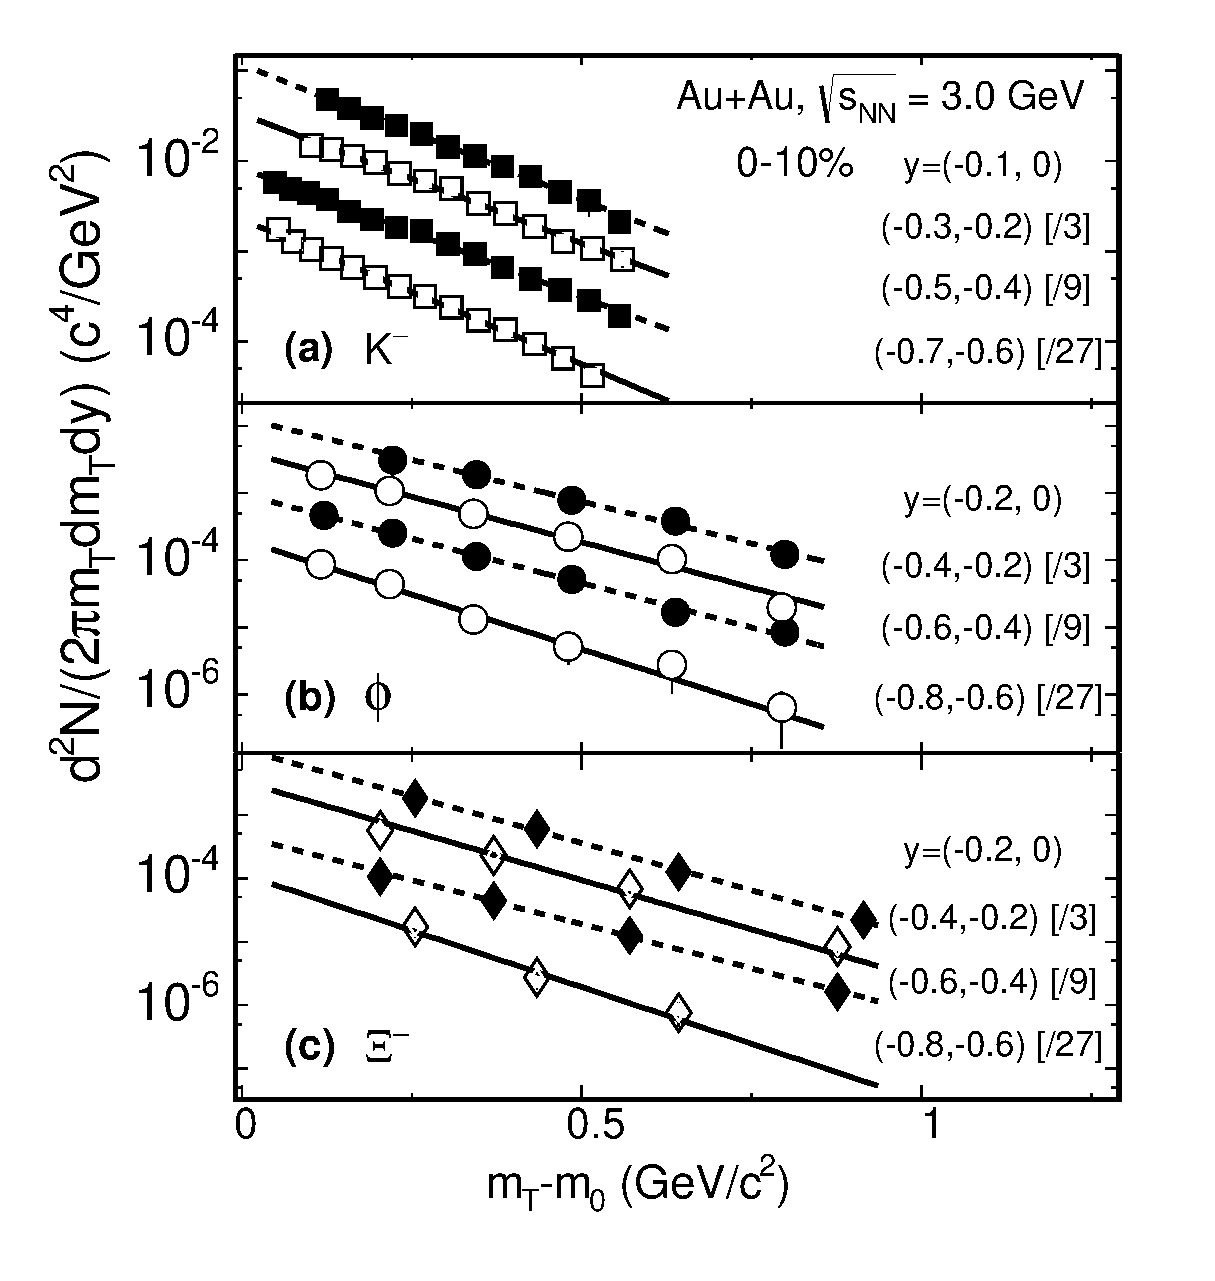
\includegraphics[width=0.41\textwidth]{fig/fig2_h_mT_spectra_phiMeson.eps}
  \caption{ $\phi$-meson and $K^-$ invariant yield as a function of transverse kinetic energy ($m_T-m_0$) for various rapidity regions in 0-10\% central Au+Au collisions at ${\sqrt{s_{\rm NN}} = \rm{3\,GeV}}$. Solid and dashed black lines depict exponential function fits to the measured data points.}
\label{fig:phimTSpectra} 
\end{figure}

\begin{figure*}
\centering
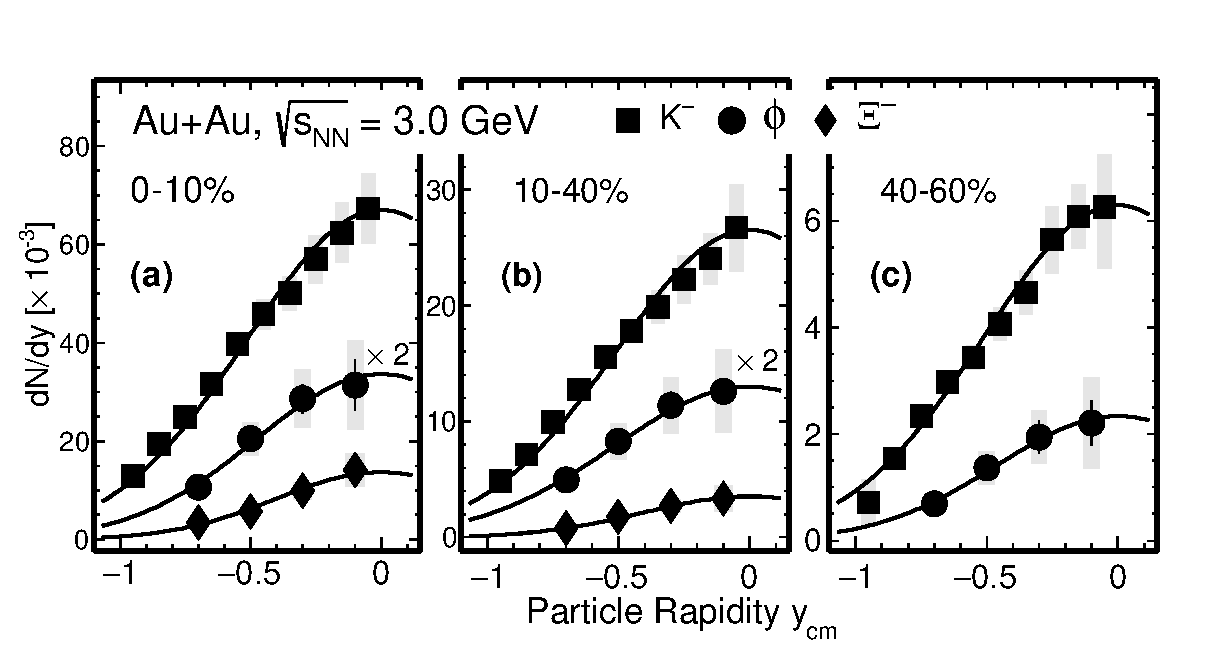
\includegraphics[width=0.8\textwidth]{fig/fig3_dndy.eps}
  \caption{ Rapidity distributions of $K^-$ (squares) and $\phi$-meson (circles) $p_T$-integrated yields $dN/dy$ in 0-10\% (a), 10-40\% (b) and 40-60\% (c) Au+Au collisions at ${\sqrt{s_{\rm NN}} = \rm{3\,GeV}}$. The full symbols show the measured data, while the open ones are reflected data with respect to $y=0$ in the center-of-mass frame. Solid lines depict Gaussian function fits to the data points.}
\label{fig:phiYSpectra} 
\end{figure*}


\begin{figure}
\centering
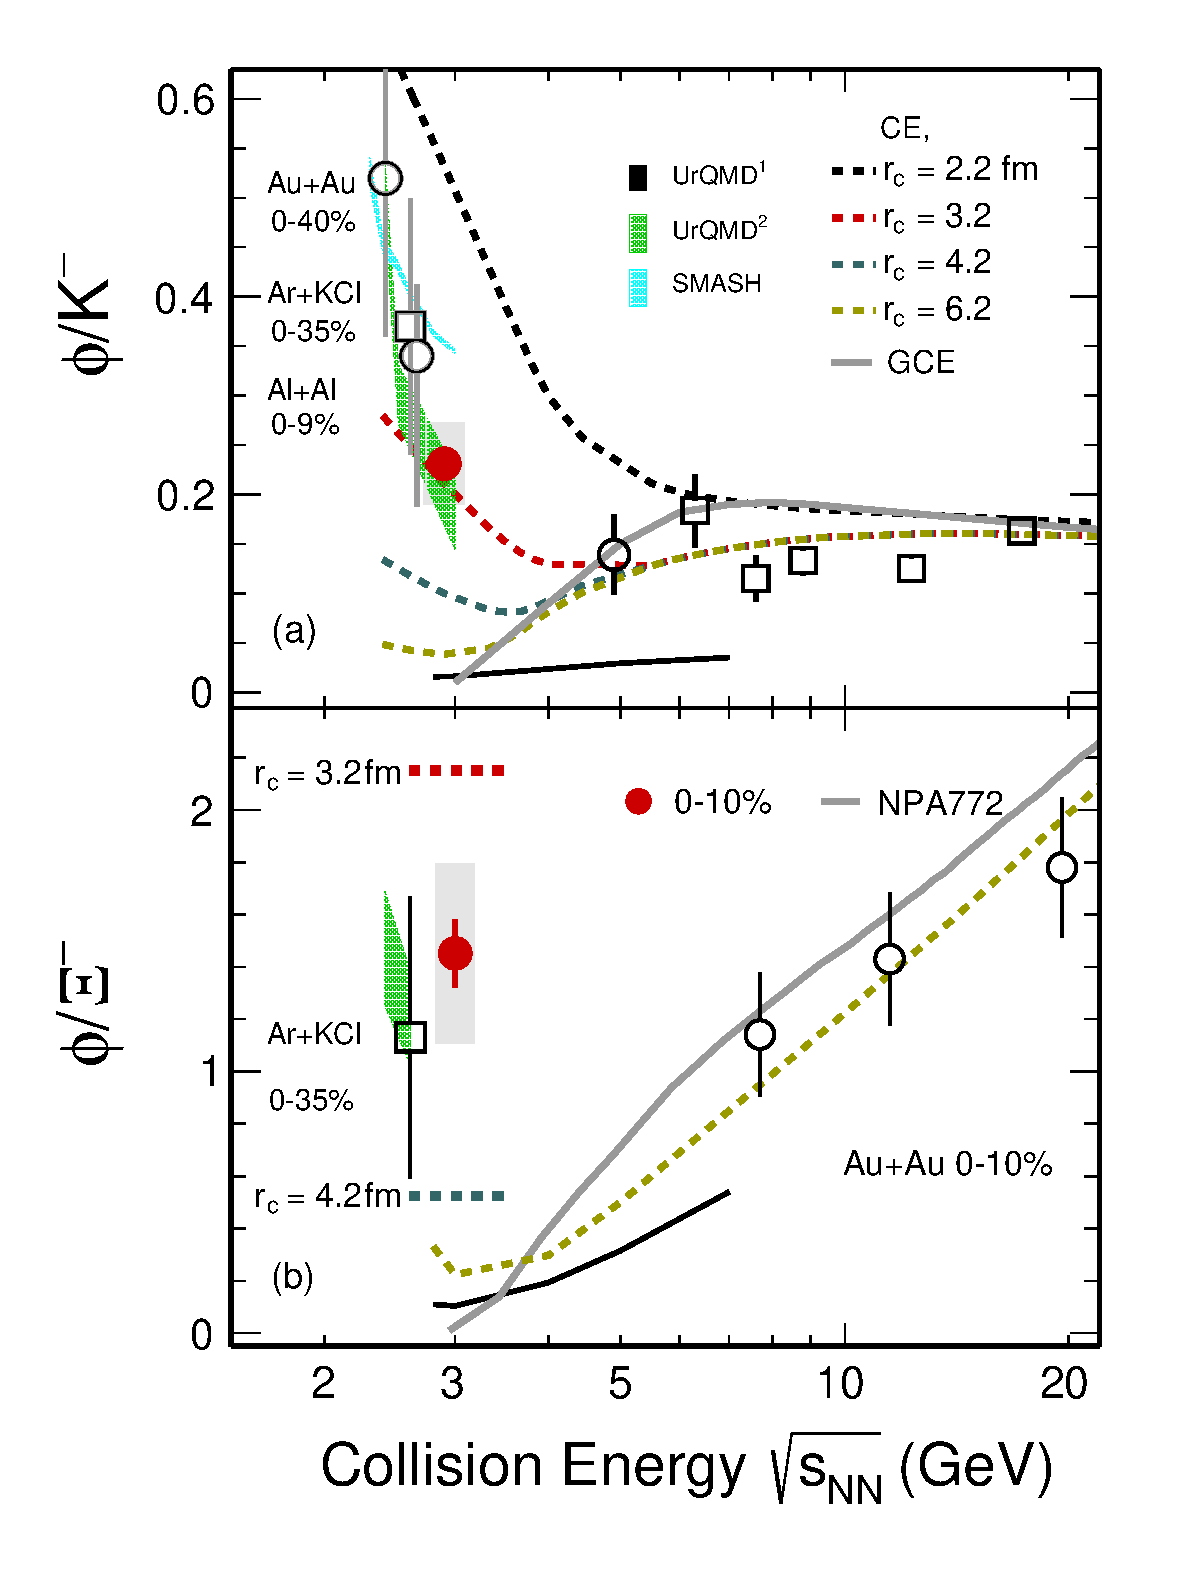
\includegraphics[width=0.41\textwidth]{fig/fig4_phi_over_kminus_zoomin.eps}
  \caption{ $\phi/K-$ ratio as a function of collision energy $\sqrt{s_{\rm NN}}$. The colored full symbols show these measurements in three centrality bins, whereas the other data points represented by different markers from various energies and collision system. The red arrow depict the $\phi$-meson production threshold in proton-proton collisions. The grey solid line represents a thermal model calculation based on grand canonical ensemble (GCE) while the dotted lines depict these calculations based on canonical ensemble (CE) with four different parameters of strangeness correlation radius ($r_c$).}
\label{fig:phi2Kratio} 
\end{figure}

Compare to models ...


In summary ...



% Chapter acknowledgement
%\section{Acknowledgement}
%\label{acknowledgement}

We thank the RHIC Operations Group and RCF at BNL, the NERSC Center at LBNL, and the Open Science Grid consortium for providing resources and support. This work is supported in part by the Office of Nuclear Physics within the U.S. DOE Office of Science, the U.S. National Science Foundation, the Ministry of Education and Science of the Russian Federation, National Natural Science Foundation of China, Chinese Academy of Science, the Ministry of Science and Technology of China and the Chinese Ministry of Education, the National Research Foundation of Korea, GA and MSMT of the Czech Republic, Department of Atomic Energy and Department of Science and Technology of the Government of India; the National Science Centre of Poland, National Research Foundation, the Ministry of Science, Education and Sports of the Republic of Croatia, RosAtom of Russia and German Bundesministerium f{\"u}r Bildung, Wissenschaft, Forschung and Technologie (BMBF) and the Helmholtz Association.

\bibliography{phi3GeV}

\end{document}
%
% ****** End of file apssamp.tex ******
